\documentclass{acm_proc_article-sp}

\begin{document}

\title{Algorithmic and Economic Aspects of the Internet}
%
% You need the command \numberofauthors to handle the 'placement
% and alignment' of the authors beneath the title.
%
% For aesthetic reasons, we recommend 'three authors at a time'
% i.e. three 'name/affiliation blocks' be placed beneath the title.
%
% NOTE: You are NOT restricted in how many 'rows' of
% "name/affiliations" may appear. We just ask that you restrict
% the number of 'columns' to three.
%
% Because of the available 'opening page real-estate'
% we ask you to refrain from putting more than six authors
% (two rows with three columns) beneath the article title.
% More than six makes the first-page appear very cluttered indeed.
%
% Use the \alignauthor commands to handle the names
% and affiliations for an 'aesthetic maximum' of six authors.
% Add names, affiliations, addresses for
% the seventh etc. author(s) as the argument for the
% \additionalauthors command.
% These 'additional authors' will be output/set for you
% without further effort on your part as the last section in
% the body of your article BEFORE References or any Appendices.

\numberofauthors{2} %  in this sample file, there are a *total*
% of EIGHT authors. SIX appear on the 'first-page' (for formatting
% reasons) and the remaining two appear in the \additionalauthors section.
%
\author{
% You can go ahead and credit any number of authors here,
% e.g. one 'row of three' or two rows (consisting of one row of three
% and a second row of one, two or three).
%
% The command \alignauthor (no curly braces needed) should
% precede each author name, affiliation/snail-mail address and
% e-mail address. Additionally, tag each line of
% affiliation/address with \affaddr, and tag the
% e-mail address with \email.
%
% 1st. author
\alignauthor
Sam Phippen\titlenote{sp9857}\\
       \email{samphippen@googlemail.com}
% 2nd. author
\alignauthor
Luke Murray\titlenote{lm9131}
       \email{lm9131@bris.ac.uk}
}
% There's nothing stopping you putting the seventh, eighth, etc.
% author on the opening page (as the 'third row') but we ask,
% for aesthetic reasons that you place these 'additional authors'
% in the \additional authors block, viz.
% Just remember to make sure that the TOTAL number of authors
% is the number that will appear on the first page PLUS the
% number that will appear in the \additionalauthors section.

\maketitle
\begin{abstract}

For the assignment we attempted to implement the Adaptive
Aggressive\cite{Vytellingum:AA} trading agent strategy. Even with corrections
emailed by D. Cliff we found that our strategy does not trade as efficiently as
is implied in other background research\cite{DC:dominate}. In this paper we've
done a comparative analysis of the existing trading agents provided in BSE,
along with our implementation. We have also performed a post mortem analysis as
to why we believe that our trader is not trading as efficiently as expected.

We had initially set our sights on taking an implementation of AA and trying to
improve upon it, with a view to building something new and potentially more
effective, however, having found ourselves in a position where the agent is
nowhere near as effective as we expected, this was not a good springboard for
extension.

\end{abstract}

\section{Analysis of our agent with existing traders}

\subsection {Many versus many tests} For the analysis we started with a many
versus many test of our implementation versus each of the agents provided with
BSE. In this experiment we used the stepped supply and demand schedule provided
with an early version of the Bristol Stock Exchange, with three distinct time
periods, the first having prices in the range 10-190, the second in the range
200-300 and the third having prices in the same range as the first. In the many
versus many test 20 agents of each type were used (10 sellers and 10 buyers),
and the tests with this supply and demand schedule were repeated a total of 25
times.

The table below shows the number of rounds that our agent lost, the mean
difference in profit between the other agent and ours, and the standard
deviation of the difference in profit also.

\begin{center}
  \begin{tabular}{ l | l | l | l }
        Agent Type & Tests lost & $\Delta$ Profit Mean & $\Delta$ Profit StDev \\\hline
        Giveaway & 24 & 63.84 & 34.16\\
        ZIC & 25 & 75.38 & 36.15\\
        Shaver & 25 & 95.63 & 21.01\\
        Sniper & 25 & 22.67 & 12.78\\
        ZIP & 25 & 97.08 & 41.38\\
  \end{tabular}
\end{center}

In almost all of these cases our agent consistently generated a profit,
however when run against the Shaver agent, an oddity occurred. The agent on
average generated a loss which can be seen on the box plot in figure 1.

\begin{figure}[h!] 
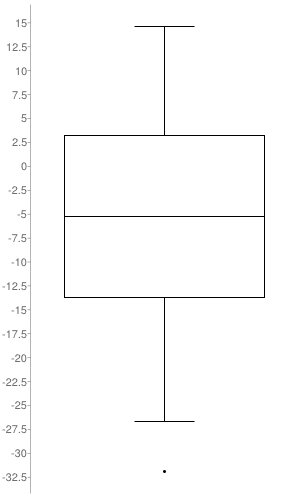
\includegraphics[width=80mm]{box-plot-image.png}

\caption{Box plot of average profits of the 20 AA agents implemented by us in
the many vs many test against shaver agents. Box plot generated from:
http://www.alcula.com/calculators/statistics/box-plot/}
\end{figure}

-- insert explanation about that here.

\subsection{1 v 1 tests} Given these initially dismal results, we decided that
a good place to start a detailed analysis would be a 1v1 test with the Giveaway
trader, which is clearly the worst of all the traders within the BSE system.
300 1v1 tests were performed, we used the same schedule as the many versus many
test, with a longer total trading time of 1800. Results where both bots made
zero profit were eliminated, this brought the number of tests included for
analysis down from 300 to 242. Of these tests 103 were won by Giveaway and 139
were won by our agent. The distributions of profit for each agent, as well as
the distribution of differences in profit can be seen in figures 2 and 3.

\begin{figure}[h!] 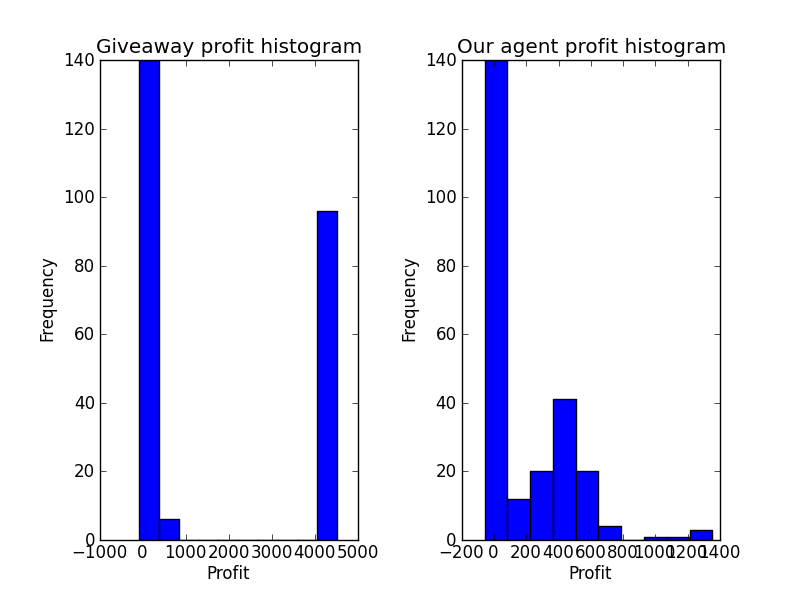
\includegraphics[width=80mm]{giveaway_1_v_1.png}
\caption{Histogram of profit distributions over 300 similar trading runs for
the two bot types used in the 1v1 test. Note axis are different for the two
bots} \end{figure}

\begin{figure}[h!] 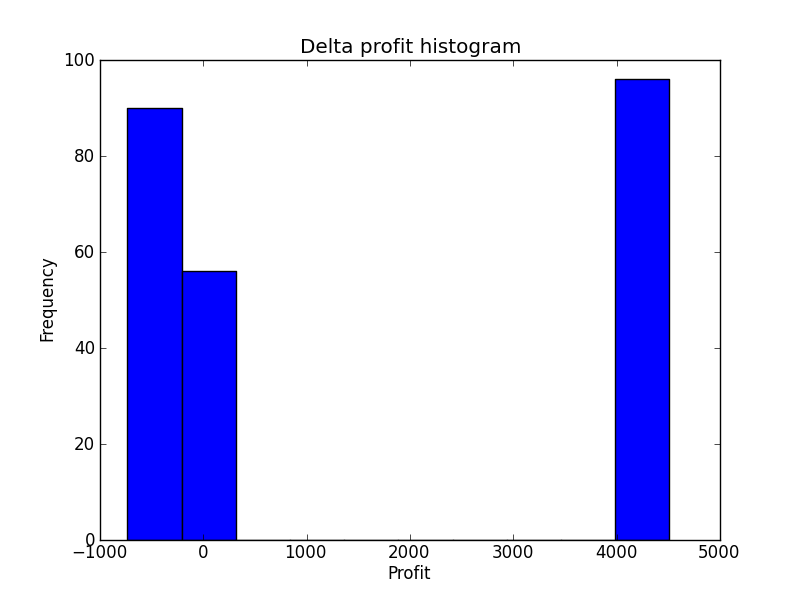
\includegraphics[width=80mm]{giveaway_1_v_1_delta.png}
\caption {Histogram showing the difference between Giveaway and our AA implementation,
positive profit represents cases where Giveaway made more profit than AA}
\end{figure}

\newpage
Upon initially inspecting these graphs we had assumed that our agent should
lose to Giveaway, however we checked the medians of the distributions and noted
that the median profit of the Giveaway agent (1.7) was less than the median
profit (50.0) of our agent. We feel that this difference in profits is the
reason for our agent's overall victory against Giveaway. To determine if the
difference in medians is significant we decided to use the Wilcoxon signed-rank
test\cite{wiki:wilcoxon}. We like this test because:

\begin{enumerate}
\item It makes no assumptions about the underlying
distribution of profit pairs, as we can see from the histogram, these are
nowhere near normally distributed.

\item It handles the fact that the pairs are dependant but the individual runs
are independent.

\item We feel that the assumptions the distribution makes are fulfilled here:
the pairs do come from the same distributions. The pairs have been generated
largely at random by running different tests and collecting results. The data
are obviously ordinal as they are floating amounts of profit.

\end{enumerate}

In order to conduct this test we represented each run as a pair of
$(profit_{giveaway}, profit_{agent})$. The profits in the pair are taken from
the average profit column in the output of running BSE. This means that in
reality the profit values are divided through by two for each agent, as it is
the average of 1 seller and 1 buyer in each case. This does not affect the test
because the change in magnitude is the same for both agents.

The test runs over the difference between the first and second value in the
pair. Our null hypothesis $H0$ is that the median difference of each pair is
zero, with our positive hypothesis $H1$ being that the median difference of
each pair is not zero. We performed the test using scipy's built in Wilcoxon
signed-rank test implementation\cite{scipy:wilcoxon} and the results were
conclusive.  With $p=1.2\times10^{-6}$ we reject $H0$ and conclude
that the difference in medians is significant, as such the difference in
profits generated is statistically significant.

This test was repeated for each of ZIC, Shaver, Sniper and ZIP. In each case,
the results were that, our agent performed worse than the other
agent with our agent having a lower median score and the Wilcoxon test giving
p < 0.01 in each case.

In light of the test against Giveaway it is  worth noting the spike at a profit
of around ~4000 in figure 3.  These occasions correspond to Giveaway making
4000 more profit than our agent. A quick analysis of the data indicates that
nearly all of these occur when our agent issues no trades (zero balance at the
end of trading). As such we concluded that for whatever reason on these events
(96/242 runs) the conditions never reach the point where our agent starts
trading. This is not unreasonable given the warmup period of the algorithm and
the low number of traders in the system.

\subsection{Experiments with supply and demand schedules}

We wanted to determine under what, if any, supply and demand conditions our
agent could outperform some of the better algorithms in the system. In order to
do this we conducted several experiments with varying supply and demand
schedules listed below. We use n=300 as our number of trials, 1 v 1 tests and a
total time period length of 1800. Initially all tests were performed against
ZIC

\subsection{Totally open market}

In this set of trials we used the hard limits of BSE, minimum price of 1 and
maximum price of 1000 for both the supply and demand curves, for the entire
time range, using a drip-poisson timemode with a 30 second replenishment time.
The idea behind this experiment is to gather an understanding as to how our
agent performs in a totally unconstrained environment.

%
% The following two commands are all you need in the
% initial runs of your .tex file to
% produce the bibliography for the citations in your paper.
\bibliographystyle{abbrv}
\bibliography{paper}  % sigproc.bib is the name of the Bibliography in this case
% You must have a proper ".bib" file
%  and remember to run:
% latex bibtex latex latex
% to resolve all references
%
% ACM needs 'a single self-contained file'!
%
%APPENDICES are optional
%\balancecolumns
\appendix
\end{document}
